\documentclass[12pt,a4paper]{article}
\usepackage{geometry}
\usepackage{slashbox}
\geometry{
	a4paper,
	total={170mm,257mm},
	left=20mm,
	right=20mm,
	top=20mm,
	bottom=20mm
}
\usepackage{graphicx}
\usepackage{pdfpages}
\usepackage{placeins}
\usepackage{float}

\usepackage{polski}
\usepackage[utf8]{inputenc}

\begin{document}
	
	\begin{titlepage}
		\newgeometry{top=5.5cm, bottom=3cm}
		
		\centering
		{\huge\bfseries Logika układów cyfrowych lab.\par}
		
		\vspace{0.5cm}
		Prowadzący: Mgr inż. Antoni Sterna (E02-38m, wtorek 17:05) \\
	
		\vspace{1.1cm}
		{\Large sprawozdanie 5 - 2017.11.14\par}
		\vfill
		
		{\large\bfseries Jakub Dorda 235013\par}
		{\large\bfseries Marcin Kotas 235098\par}
		
		\vspace{1cm}
		\today \\ \LaTeX
		
		\restoregeometry
	\end{titlepage}

	\newgeometry{top=1.5cm, bottom=1.5cm, left=20mm, right=20mm}

	\section{Wprowadzenie/cel ćwiczeń}
	
		Celem ćwiczeń było poznanie podstaw projektowania automatów w wariantach Moore'a i Mealy. Należało zaprojektować grafy w obu wariantach dla subtraktora szeregowego oraz komparatora szeregowego. Dodatkowo przeprowadzona została synteza strukturalna komparatora w wariancie Mealy w celu uruchomienia go na zestawie UNILOG.
		
		
	\section{Subtraktor szeregowy}
	
		\subsection{Automat Moore'a}
		
			\begin{itemize}
				\item Wejścia: \(Z = \{Z_0, Z_1, Z_2, Z_3\}\)\\
				
				\begin{minipage}{{.5\textwidth}}
					\centering
					\begin{tabular}{r|cc}
						&	\(z_1\)	&	\(z_0\)\\\hline
						\(Z_0\)	&	0	&	0	\\
						\(Z_1\)	&	0	&	1	\\
						\(Z_2\)	&	1	&	0	\\
						\(Z_3\)	&	1	&	1	\\
					\end{tabular}
				\end{minipage}%
				\begin{minipage}{{.5\textwidth}}
					\(z_1\) - cyfra odjemnej\\
					\(z_0\) - cyfra odjemnika
				\end{minipage}
			
				\item Stany wewnętrzne: \(Q =\{Q_0, Q_1, Q_2, Q_3\}\)\\
					
					\begin{minipage}{{.5\textwidth}}
						\centering
						\begin{tabular}{r|cc}
							&	\(q_1\)	&	\(q_0\)\\\hline
							\(Q_0\)	&	0	&	0	\\
							\(Q_1\)	&	0	&	1	\\
							\(Q_2\)	&	1	&	0	\\
							\(Q_3\)	&	1	&	1	\\
						\end{tabular}
					\end{minipage}%
					\begin{minipage}{{.5\textwidth}}	
						\(Q_0\) - stan bez pożyczki, wynik = 0\\
						\(Q_1\) - stan z pożyczką, wynik = 0\\
						\(Q_2\) - stan bez pożyczki, wynik = 1\\
						\(Q_3\) - stan z pożyczką, wynik = 1
					\end{minipage}
				
				\item Funkcja wyjść: \(Y=\{Y_0, Y_1\}\)\\
				
					\begin{minipage}{{.5\textwidth}}
						\centering
						\begin{tabular}{r|c}
							\(Q\)	&	\(Y\)	\\\hline
							\(Q_0\)	&	\(Y_0\)	\\
							\(Q_1\)	&	\(Y_0\)	\\
							\(Q_2\)	&	\(Y_1\)	\\
							\(Q_3\)	&	\(Y_1\)	\\
						\end{tabular}
					\end{minipage}%
					\begin{minipage}{{.5\textwidth}}	
						\(Y_0\) - wynik = 0\\
						\(Y_1\) - wynik = 1
					\end{minipage}
			\end{itemize}
			
			\begin{figure}[H]
				\centering
				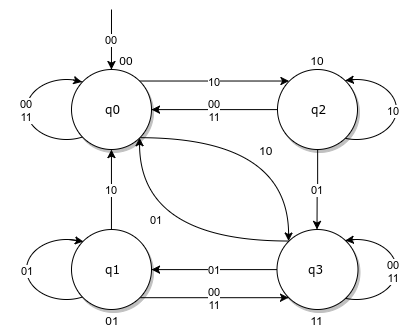
\includegraphics[width=.5\textwidth]{schem/diag1.png}
				\\
				\vspace{.1cm}
				Graf 1 - subtraktor szeregowy w wersji Moore'a
			\end{figure}
			
			%\begin{center}
			%	\makebox[\textwidth]{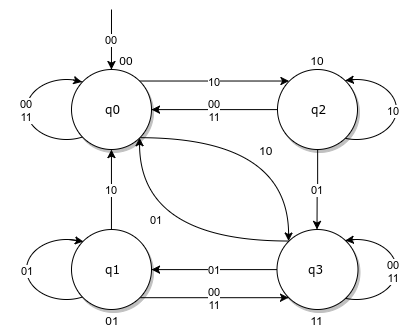
\includegraphics[width=\paperwidth - 86mm]{schem/diag1.png}}
			%	Graf 1 - subtraktor szeregowy w wersji Moore'a
			%\end{center}
			
			
		\subsection{Automat Mealy}
			\begin{itemize}
				\item Wejścia: \(Z = \{Z_0, Z_1, Z_2, Z_3\}\)\\
				
				\begin{minipage}{{.5\textwidth}}
					\centering
					\begin{tabular}{r|cc}
						&	\(z_1\)	&	\(z_0\)\\\hline
						\(Z_0\)	&	0	&	0	\\
						\(Z_1\)	&	0	&	1	\\
						\(Z_2\)	&	1	&	0	\\
						\(Z_3\)	&	1	&	1	\\
					\end{tabular}
				\end{minipage}%
				\begin{minipage}{{.5\textwidth}}	
					
					\(z_1\) - cyfra odjemnej\\
					\(z_0\) - cyfra odjemnika
				\end{minipage}
				
				\item Stany wewnętrzne: \(Q =\{Q_0, Q_1\}\)
					
					\(Q_0\) - stan bez pożyczki\\
					\(Q_1\) - stan z pożyczką
					
				\item Funkcja wyjść: \(Y=\{Y_0, Y_1\}\)
					
					\(Y_0\) - wynik = 0\\
					\(Y_1\) - wynik = 1
			\end{itemize}
			
			\begin{figure}[H]
				\centering
				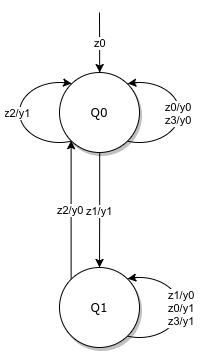
\includegraphics[width=.25\textwidth]{schem/diag2.png}
				\\
				\vspace{.1cm}
				Graf 2 - subtraktor szeregowy w wersji Mealy
			\end{figure}
		
			%\begin{center}
			%	\makebox[\textwidth]{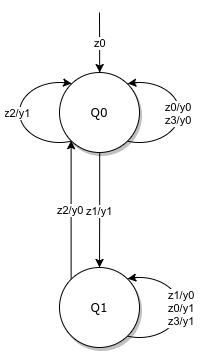
\includegraphics[width=\paperwidth - 145mm]{schem/diag2.png}}
			%	Graf 2 - subtraktor szeregowy w wersji Mealy
			%\end{center}
		
	\section{Komparator szeregowy}
	
		\subsection{Automat Moore'a}
		
		\begin{itemize}
			\item Wejścia: \(Z = \{Z_0, Z_1, Z_2, Z_3\}\)\\
			
			\begin{minipage}{{.5\textwidth}}
				\centering
				\begin{tabular}{r|cc}
					&	\(z_1\)	&	\(z_0\)\\\hline
					\(Z_0\)	&	0	&	0	\\
					\(Z_1\)	&	0	&	1	\\
					\(Z_2\)	&	1	&	0	\\
					\(Z_3\)	&	1	&	1	\\
				\end{tabular}
			\end{minipage}%
			\begin{minipage}{{.5\textwidth}}
				\(z_1\) - cyfra pierwszej liczby\\
				\(z_0\) - cyfra drugiej liczby
			\end{minipage}
			
			\newpage
			\item Stany wewnętrzne: \(Q =\{Q_1, Q_2, Q_3\}\)\\
			
			\begin{minipage}{{.5\textwidth}}
				\centering
				\begin{tabular}{r|cc}
					&	\(q_1\)	&	\(q_0\)\\\hline
					\(Q_1\)	&	0	&	1	\\
					\(Q_2\)	&	1	&	0	\\
					\(Q_3\)	&	1	&	1	\\
				\end{tabular}
			\end{minipage}%
			\begin{minipage}{{.5\textwidth}}	
				\(Q_1\) - druga liczba większa\\
				\(Q_2\) - pierwsza liczba większa\\
				\(Q_3\) - stan wejściowy, obie liczby równe\\
			\end{minipage}
			
			\item Funkcja wyjść: \(Y=\{Y_1, Y_2, Y_3\}\) (kodowanie \(y_1,y_0\) takie samo jak dla stanów wew.)\\
			
			\begin{minipage}{{.5\textwidth}}
				\centering
				\begin{tabular}{r|c}
					\(Q\)	&	\(Y\)	\\\hline
					\(Q_1\)	&	\(Y_1\)	\\
					\(Q_2\)	&	\(Y_2\)	\\
					\(Q_3\)	&	\(Y_3\)	\\
				\end{tabular}
			\end{minipage}%
			\begin{minipage}{{.5\textwidth}}	
				\(Y_1\) - druga liczba większa\\
				\(Y_2\) - pierwsza liczba większa\\
				\(Y_3\) - obie liczby równe\\
			\end{minipage}
		\end{itemize}\vspace{1.5cm}
		
		\begin{figure}[H]
			\centering
			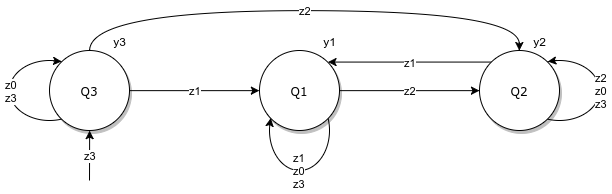
\includegraphics[width=.75\textwidth]{schem/diag3.png}
			\\
			\vspace{.1cm}
				Graf 3 - komparator szeregowy w wersji Moore'a
		\end{figure}
	
		%\begin{center}
		%	\makebox[\textwidth]{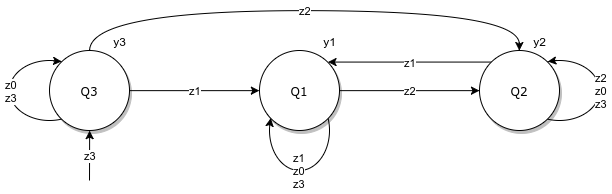
\includegraphics[width=\paperwidth - 20mm]{schem/diag3.png}}
		%	Graf 3 - komparator szeregowy w wersji Moore'a
		%\end{center}	
		
		\subsection{Automat Mealy}
		\begin{itemize}
			\item Wejścia oraz stany wewnętrzne takie same jak dla automatu Moore'a
			
			\item Wyjścia: \(Y=\{Y_1, Y_2, Y_3\}\)\\
			
			\begin{minipage}{{.5\textwidth}}
				\centering
				\begin{tabular}{r|cc}
					&	\(y_1\)	&	\(y_0\)\\\hline
					\(Y_1\)	&	0	&	1	\\
					\(Y_2\)	&	1	&	0	\\
					\(Y_3\)	&	1	&	1	\\
				\end{tabular}
			\end{minipage}%
			\begin{minipage}{{.5\textwidth}}	
				\(Y_1\) - druga liczba większa\\
				\(Y_2\) - pierwsza liczba większa\\
				\(Y_3\) - obie liczby równe\\
			\end{minipage}
		\end{itemize}
		
		\begin{figure}[H]
			\centering
			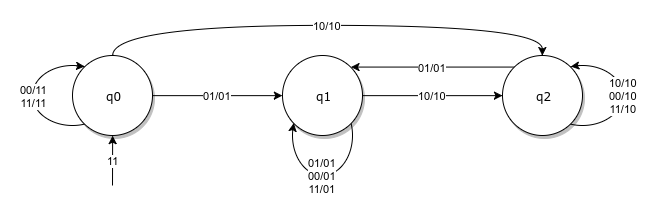
\includegraphics[width=.75\textwidth]{schem/diag4.png}
			\\
			\vspace{.1cm}
			Graf 4 - komparator szeregowy w wersji Mealy
		\end{figure}
	
		%\begin{center}
		%	\makebox[\textwidth]{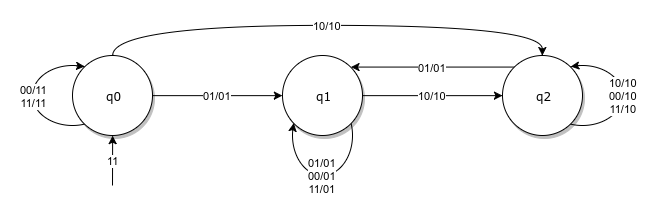
\includegraphics[width=\paperwidth - 20mm]{schem/diag4.png}}
		%	Graf 4 - komparator szeregowy w wersji Mealy
		%\end{center}	
	
		\subsection{Tabela prawdy i tablice Karnaugh dla automatu Mealy:}
			\begin{table}[H]
			\begin{minipage}{.5\textwidth}
				\caption{Tabela Prawdy - funkcja przejść}
				\vspace{0.2cm}
				\centering
				\begin{tabular}{cccc|cc}
					\multicolumn{4}{c|}{\(t\)}	&	\multicolumn{2}{c}{\(t+1\)} \\
					\(q_1\)&\(q_0\)&\(z_1\)&\(z_0\)&\(q_1\)&\(q_0\)\\\hline
					0	&	0	&	0	&	0	&	-	&	-	\\
					0	&	0	&	0	&	1	&	-	&	-	\\
					0	&	0	&	1	&	0	&	-	&	-	\\
					0	&	0	&	1	&	1	&	-	&	-	\\\hline
					0	&	1	&	0	&	0	&	0	&	1	\\
					0	&	1	&	0	&	1	&	0	&	1	\\
					0	&	1	&	1	&	0	&	1	&	0	\\
					0	&	1	&	1	&	1	&	0	&	1	\\\hline
					1	&	0	&	0	&	0	&	1	&	0	\\
					1	&	0	&	0	&	1	&	0	&	1	\\
					1	&	0	&	1	&	0	&	1	&	0	\\
					1	&	0	&	1	&	1	&	1	&	0	\\\hline
					1	&	1	&	0	&	0	&	1	&	1	\\
					1	&	1	&	0	&	1	&	0	&	1	\\
					1	&	1	&	1	&	0	&	1	&	0	\\
					1	&	1	&	1	&	1	&	1	&	1	\\
				\end{tabular}
			\end{minipage}%
			\begin{minipage}{.5\textwidth}
				\caption{Tablica Karnaugh dla $q_1$}
				\vspace{0.2cm}
				\centering
				\begin{tabular}{c|c|c|c|c}
					\backslashbox{$z_1z_0$}{$q_1q_0$}&00&01&11&10\\\hline
					00	&	-	&	0	&	1	&	1	\\\hline
					01	&	-	&	0	&	0	&	0	\\\hline
					11	&	-	&	0	&	1	&	1	\\\hline
					10	&	-	&	1	&	1	&	1	
				\end{tabular}
				\vspace{1cm}
				
				\caption{Tablica Karnaugh dla $q_0$}
				\vspace{0.2cm}
				\centering
				\begin{tabular}{c|c|c|c|c}
					\backslashbox{$z_1z_0$}{$q_1q_0$}&00&01&11&10\\\hline
					00	&	-	&	1	&	1	&	0	\\\hline
					01	&	-	&	1	&	1	&	1	\\\hline
					11	&	-	&	1	&	1	&	0	\\\hline
					10	&	-	&	0	&	0	&	0	
				\end{tabular}
			\end{minipage}
			\end{table}
		
			\begin{table}[H]
			\begin{minipage}{.5\textwidth}
				\caption{Tabela Prawdy - funkcja wyjść}
				\vspace{0.2cm}
				\centering
				\begin{tabular}{cccc|cc}
					\(q_1\)&\(q_0\)&\(z_1\)&\(z_0\)&\(y_1\)&\(y_0\)\\\hline
					0	&	0	&	0	&	0	&	-	&	-	\\
					0	&	0	&	0	&	1	&	-	&	-	\\
					0	&	0	&	1	&	0	&	-	&	-	\\
					0	&	0	&	1	&	1	&	-	&	-	\\\hline
					0	&	1	&	0	&	0	&	0	&	1	\\
					0	&	1	&	0	&	1	&	0	&	1	\\
					0	&	1	&	1	&	0	&	1	&	0	\\
					0	&	1	&	1	&	1	&	0	&	1	\\\hline
					1	&	0	&	0	&	0	&	1	&	0	\\
					1	&	0	&	0	&	1	&	0	&	1	\\
					1	&	0	&	1	&	0	&	1	&	0	\\
					1	&	0	&	1	&	1	&	1	&	0	\\\hline
					1	&	1	&	0	&	0	&	1	&	1	\\
					1	&	1	&	0	&	1	&	0	&	1	\\
					1	&	1	&	1	&	0	&	1	&	0	\\
					1	&	1	&	1	&	1	&	1	&	1	\\
				\end{tabular}
			\end{minipage}%
			\begin{minipage}{.5\textwidth}
				\caption{Tablica Karnaugh dla $y_1$}
				\vspace{0.2cm}
				\centering
				\begin{tabular}{c|c|c|c|c}
					\backslashbox{$z_1z_0$}{$q_1q_0$}&00&01&11&10\\\hline
					00	&	-	&	0	&	1	&	1	\\\hline
					01	&	-	&	0	&	0	&	0	\\\hline
					11	&	-	&	0	&	1	&	1	\\\hline
					10	&	-	&	1	&	1	&	1	
				\end{tabular}
				\vspace{1cm}
				
				\caption{Tablica Karnaugh dla $y_0$}
				\vspace{0.2cm}
				\centering
				\begin{tabular}{c|c|c|c|c}
					\backslashbox{$z_1z_0$}{$q_1q_0$}&00&01&11&10\\\hline
					00	&	-	&	1	&	1	&	0	\\\hline
					01	&	-	&	1	&	1	&	1	\\\hline
					11	&	-	&	1	&	1	&	0	\\\hline
					10	&	-	&	0	&	0	&	0	
				\end{tabular}
			\end{minipage}
			\end{table}
		
		\subsection{Minimalizacje:}
			\begin{displaymath}
			q_1(t+1) = y_1 = z_1\bar{z_0} + q_1z_1 + q_1\bar{z_0}= \overline{\overline{z_1\bar{z_0}} \cdot \overline{q_1z_1} \cdot \overline{q_1\bar{z_0}}}
			\end{displaymath}
			\begin{displaymath}
			q_0(t+1) = y_0 = \bar{z_1}z_0 + q_0\bar{z_1} + q_0z_0= \overline{\overline{\bar{z_1}z_0} \cdot \overline{q_0\bar{z_1}} \cdot \overline{q_0z_0}}
			\end{displaymath}
		
		\newpage
		\subsection{Użyte wzory:}
			\begin{equation}
			\overline{a+b}=\bar{a}\cdot\bar{b}
			\end{equation}
		
		\subsection{Schemat układu:}
		
		\vspace{1.5cm}
		\begin{center}
			\makebox[\textwidth]{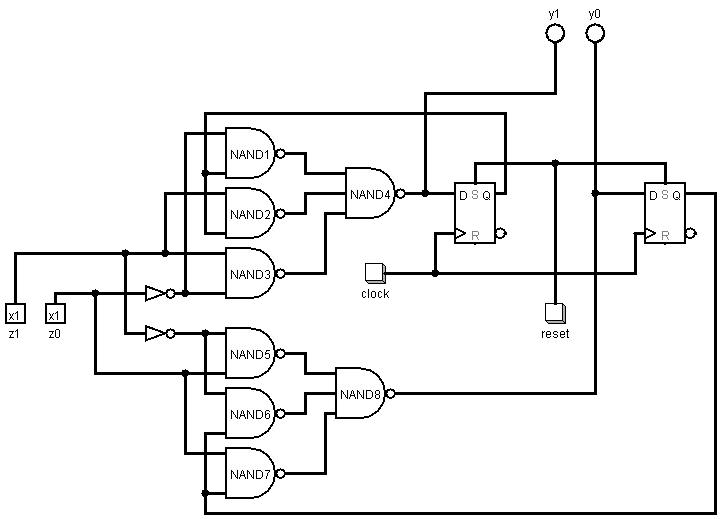
\includegraphics[width=\paperwidth - 30mm]{schem/circuitv2.png}}
			Schemat 1 - komparator szeregowy w wersji Mealy
		\end{center}

	\section{Wnioski/podsumowanie}
	
			W celu sprawdzenia poprawności działania komparatora należało przeprowadzić testy dla wszystkich możliwych kombinacji wejść oraz stanów. Za stan wejściowy przyjęto \(q_1=1, q_0 = 1\), więc przycisk reset należało podłączyć do wejść set przerzutników.
	
\end{document}